% Drawing 154/07-24 -- folder 154, batch 07, archive page 134 (PDF page 135).
% Transcription: colonne de droite : deux dessins en couleur. Un fuseau bordé de tirets vert clair et d'un trait vert clair, entre deux croisements orange, balayé d'une courbe au crayon qui revient sur elle-même, une flèche vers la droite ; un fuseau semblable, bordé de tirets vert clair et vert foncé, prolongé des deux côtés par une droite noire, les sommets marqués $a$ (avec l'orientation $\omega_a$) et $b$ (avec $\omega_b$), de petites flèches de rotation
% Kind: two spindles between two crossings. Method 2 (schematic redraw from the facsimile). Status: partial.
% Notes: Upper drawing: a solid light green stroke (the lower side of the spindle) and above it a line of light green dashes (the upper side); two orange crossings, each with a dark dot, the left one on the solid stroke and the right one on the dashed side; two orange strokes across the middle; a few light green dashes run from the lower left up to the left crossing; a small arrow pointing left with omega above it beside the left crossing; a black arrow to the right under the right end of the solid stroke; a thin pencil curve sweeps the spindle back and forth from left to right in loops. Lower drawing: a black line on each side, overdrawn with dark green dashes; the spindle between them, its upper side in light green dashes and its lower side in dark blue-green dashes, both over a thin pencil outline; a brown dashed median; the crossing a (dark dot) on the lower side and b on the upper side, two orange strokes between them; the arrows omega_a (to the right, under the lower side) and omega_b (to the left, above the upper side), and a curved arrow round each vertex. Crossings computed. Overlaid on the 400 dpi colour crop on 2026-11-12 and redrawn: the solid light green stroke has no arrowhead (the arrow is a separate black one), the middle strokes of the upper drawing are two, not three (the third was the pencil curve), the small arrow omega at the left crossing and the pencil curve are added, all strokes put on their ink. Still differs from the facsimile: the pencil curve is drawn as four pieces that follow its loops approximately (where it passes under the orange strokes it cannot be followed) (the small ink scribble at (31,-22) was added on 13 November). Redrawn 2026-11-12 (issue 128): to check again. Overlay check 2026-11-13 (claude-opus-5-5, issue 128): the 300 dpi colour crop laid under the redraw compiled with tectonic. The bbox cut the lower drawing (its orange strokes reach y=-78.5): enlarged to y1=0.245, same origin, so the coordinates are unchanged. Both drawings redrawn from coordinates read on 6x crops: in the upper one the solid and dashed sides, the two crossings (dots at (22.9,-25.6) and (53.5,-18)) and the six orange strokes, the omega arrow, the ink stroke over omega, the ink scribble at (31,-22) and a small dark green scribble at (17,-28.5) (both left out before), and the pen curve, now traced as one sweep of four loops that goes back over itself under the left crossing and ends in the black arrow, with a thin tail beyond it; in the lower one the two black lines, both sides of the spindle (the vertices are at (24.2,-54.2) and (73.7,-56.2)), the brown median, the four orange strokes (two through a, two through b, two between), a, b, omega_a, omega_b and the two curved arrows (the one round a was drawn on the wrong side). Still differs from the facsimile: where the pen curve passes under the orange strokes its course is interpolated, and its turn at (22.2,-33.3) and its start under the stroke at (26,-28.6) cannot be followed; the stroke over the omega of the upper drawing may be an overbar or a separate dash. 2026-11-14, Claude Opus 5.5, overlay check (issue 147): rasterised from its own coordinates over the 400 dpi colour scan (402 ppi native) on a unit grid; not compiled (no TeX in the session). Both drawings lie on their ink to within about 1 unit, the pen curve included where it can be seen; the redraw is unchanged. Still partial because the pen curve cannot be followed under the orange strokes, at its turn at (22.2,-33.3) and at its start (13 November note).
% Coordinates: 1 unit = 1 mm = 1/100 of the crop width (bbox in page fractions: [0.52, 0.085, 0.8, 0.245]; enlarged from 0.215 on 2026-11-13, the old one cut the lower drawing).
% Redrawn by Claude (claude-fable-5-2), issue #128, 2026-11-12; not checked by a human; not compiled (no TeX in the session).
% Corrected by Claude (claude-fable-5-2) 2026-11-12 (issue #128): overlaid on the 400 dpi colour facsimile and redrawn from it. Not compiled. Status: partial.
% Checked by Claude (claude-opus-5-5) 2026-11-13 (issue #128): overlaid on the 300 dpi colour facsimile and corrected; compiled with tectonic, no errors. Status: partial.
% Checked by Claude (claude-opus-5-5) 2026-11-14 (issue #147): overlaid on the 400 dpi colour facsimile; not compiled (no TeX in the session). Not checked by a human. Status: partial.
% Rights: reproduces part of the work -- behind RENDER_TRANSCRIPTS, never published by itself.
\documentclass[tikz,border=3pt]{standalone}
\usepackage{amsmath,amssymb}
\usetikzlibrary{patterns,arrows.meta}
\tikzset{Or/.style={orange!90!black}, Lg/.style={green!60!black!70}, Dg/.style={green!45!black}, Br/.style={brown!80!black}, pencil/.style={black!45}, struck/.style={black!35}, mpt/.style={circle,draw,inner sep=1.3pt}, pt/.style={circle,fill,inner sep=0.9pt}, opt/.style={circle,draw,fill=white,inner sep=1.1pt}}
\colorlet{Or}{orange!90!black}\colorlet{Ye}{yellow!80!orange}\colorlet{Lg}{green!60!black!70}\colorlet{Dg}{green!45!black}\colorlet{Br}{brown!80!black}\colorlet{Rd}{red!85!black}\colorlet{Bl}{blue!70!black}\colorlet{Gy}{black!40}
\begin{document}
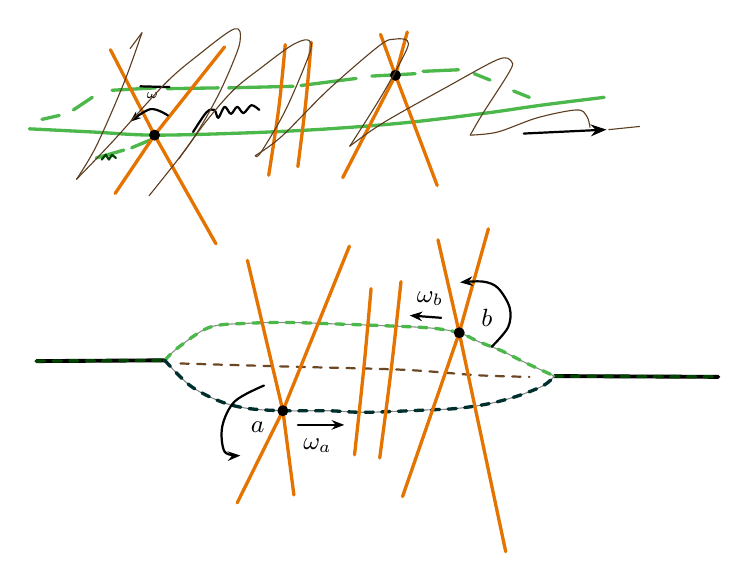
\begin{tikzpicture}[x=1mm,y=1mm,line cap=round,line join=round,font=\scriptsize]
% --- upper drawing (redrawn 2026-11-13 from the 300 dpi colour crop, extended down to 0.245) ---
\draw[Lg,very thick] plot[smooth, tension=0.55] coordinates {(7,-24.8) (15,-25.2) (22.9,-25.6) (35,-25.3) (45,-24.8) (55,-24) (65,-22.8) (72,-21.8) (80,-20.8)};
\draw[Lg,very thick] (8.6,-23.6) -- (10.8,-23.1);
\draw[Lg,very thick] (12.6,-22.4) -- (15,-20.8);
\draw[Lg,very thick] (17.5,-19.9) -- (23,-19.6);
\draw[Lg,very thick] (24.5,-19.7) -- (31,-19.6);
\draw[Lg,very thick] (32.3,-19.6) -- (40.5,-19.4);
\draw[Lg,very thick] (41.5,-19.3) -- (48.5,-18.4);
\draw[Lg,very thick] (50.5,-18.1) -- (56,-17.8);
\draw[Lg,very thick] (57,-17.5) -- (61.5,-17.3);
\draw[Lg,very thick] (63.5,-17.8) -- (65.5,-18.6);
\draw[Lg,very thick] (68.5,-20) -- (70.5,-20.8);
\draw[Lg,very thick] (15.5,-28.5) -- (19,-27.5);
\draw[Lg,very thick] (20,-27.2) -- (22.4,-26.2);
\draw[Or,very thick] (17.3,-14.75) -- (22.9,-25.6) -- (30.7,-39.4);
\draw[Or,very thick] (31.8,-14.4) -- (22.9,-25.6) -- (17.9,-33);
\draw[Or,very thick] plot[smooth, tension=0.55] coordinates {(39.5,-14.1) (38.7,-22) (37.4,-30.7)};
\draw[Or,very thick] plot[smooth, tension=0.55] coordinates {(42.8,-13.8) (42.1,-21.5) (41.1,-29.6)};
\draw[Or,very thick] (51.6,-12.8) -- (53.5,-18) -- (58.8,-32);
\draw[Or,very thick] (55,-12.5) -- (53.5,-18) -- (46.8,-31);
\draw[Dg!60!black,thick] (16.2,-28.7) -- (16.7,-28.1) -- (17.1,-28.7) -- (17.5,-28.1) -- (18,-28.5);
\node[pt,inner sep=1.4pt] at (22.9,-25.6) {};
\node[pt,inner sep=1.4pt] at (53.5,-18) {};
\draw[thick,-{Stealth[length=1.4mm]}] plot[smooth, tension=0.6] coordinates {(24.6,-23.1) (22.4,-22.3) (19.8,-23.9)};
\draw[thick] (21.1,-19.4) -- (24.8,-19.5);
\node[inner sep=0pt] at (22.6,-20.6) {\tiny $\omega$};
\draw[thick] plot[smooth, tension=0.55] coordinates {(27.8,-25.2) (29.5,-22.7) (30.5,-22.4) (31,-23.4) (31.8,-22) (32.6,-22.9) (33.4,-22) (34.2,-22.8) (35.2,-21.8) (36.2,-22.4)};
\draw[thick,-{Stealth[length=2mm]}] (69.8,-25.4) -- (80.3,-24.9);
\draw[Br!60!black,thin] (19.8,-14.6) -- (21.3,-12.6);
\draw[Br!60!black,thin] plot[smooth, tension=0.55] coordinates {(21.3,-12.6) (19,-19) (15.5,-27) (13,-31.2)};
\draw[Br!60!black,thin] plot[smooth, tension=0.55] coordinates {(13,-31.2) (17.5,-26.5) (24.4,-18.9) (29,-15) (32.3,-12.5) (33.5,-12.1) (33.8,-13) (33.4,-15) (31,-20.5) (27.5,-26.5) (22.2,-33.3)};
\draw[Br!60!black,thin] plot[smooth, tension=0.55] coordinates {(26,-28.6) (29.5,-23.8) (33,-19.8) (36.5,-17) (40,-14.4) (42,-13.5) (42.8,-14) (42.3,-16) (39.5,-22.5) (36.4,-27.8) (35.7,-28.2)};
\draw[Br!60!black,thin] plot[smooth, tension=0.55] coordinates {(35.7,-28.2) (39,-25.8) (45,-19.8) (51.5,-14.2) (53.5,-13.4) (55,-13.6) (54.8,-15) (51.8,-20.5) (47.7,-27)};
\draw[Br!60!black,thin] plot[smooth, tension=0.55] coordinates {(47.7,-27) (52,-24) (60,-19.5) (66.5,-16) (68.2,-16.2) (68,-17.5) (64.5,-23) (63,-25.6)};
\draw[Br!60!black,thin] plot[smooth, tension=0.55] coordinates {(63,-25.6) (66.5,-25.2) (71.5,-23.4) (76.5,-22.4) (77.8,-23.2) (78.2,-24.6)};
\draw[Br!60!black,thin] plot[smooth, tension=0.55] coordinates {(80.6,-24.9) (84.5,-24.5)};
% --- lower drawing ---
\draw[line width=1.4pt] (7.9,-54.3) -- (24.2,-54.2);
\draw[line width=1.4pt] (73.7,-56.2) -- (94.5,-56.3);
\draw[Dg!60!black,very thick,dashed] (7.9,-54.3) -- (24.2,-54.2);
\draw[Dg!60!black,very thick,dashed] (73.7,-56.2) -- (94.5,-56.3);
\draw[pencil,thin] plot[smooth, tension=0.55] coordinates {(24.2,-54.2) (26,-52.5) (29.9,-50) (34.7,-49.5) (40.1,-49.4) (46.5,-49.6) (52,-49.8) (58,-50.1) (61.6,-50.7) (64,-51.8) (67,-53) (70,-54.5) (73.7,-56.2)};
\draw[Lg,very thick,dashed] plot[smooth, tension=0.55] coordinates {(24.2,-54.2) (26,-52.5) (29.9,-50) (34.7,-49.5) (40.1,-49.4) (46.5,-49.6) (52,-49.8) (58,-50.1) (61.6,-50.7) (64,-51.8) (67,-53) (70,-54.5) (73.7,-56.2)};
\draw[pencil,thin] plot[smooth, tension=0.55] coordinates {(24.2,-54.2) (27.4,-57.4) (31.2,-59.4) (34.7,-60.3) (39.2,-60.6) (44.9,-60.6) (49.7,-60.8) (57.6,-60.5) (61.4,-60.3) (65.4,-59.7) (69.1,-58.7) (72.3,-57.4) (73.7,-56.2)};
\draw[Dg!70!blue!60!black,very thick,dashed] plot[smooth, tension=0.55] coordinates {(24.2,-54.2) (27.4,-57.4) (31.2,-59.4) (34.7,-60.3) (39.2,-60.6) (44.9,-60.6) (49.7,-60.8) (57.6,-60.5) (61.4,-60.3) (65.4,-59.7) (69.1,-58.7) (72.3,-57.4) (73.7,-56.2)};
\draw[Br!70!black,thick,dashed] plot[smooth, tension=0.55] coordinates {(26.2,-54.6) (40,-55) (54.5,-55.4) (64,-56.1) (70.5,-56.3)};
\draw[Or,very thick] (34.7,-41.5) -- (39.2,-60.6) -- (40.6,-71.3);
\draw[Or,very thick] (47.65,-39.7) -- (39.2,-60.6) -- (33.4,-72.3);
\draw[Or,very thick] plot[smooth, tension=0.55] coordinates {(50.4,-45.1) (49.5,-55) (48.3,-66.2)};
\draw[Or,very thick] plot[smooth, tension=0.55] coordinates {(54.2,-44.2) (53,-55) (51.5,-66.6)};
\draw[Or,very thick] (58.9,-38.9) -- (61.6,-50.7) -- (67.5,-78.5);
\draw[Or,very thick] (65.3,-37.5) -- (61.6,-50.7) -- (54.4,-71.5);
\node[pt,inner sep=1.4pt] at (39.2,-60.6) {};
\node[pt,inner sep=1.4pt] at (61.6,-50.7) {};
\node[inner sep=1pt] at (36,-62.7) {\small $a$};
\draw[thick,-{Stealth[length=1.6mm]}] (41.1,-62.4) -- (47,-62.4);
\node[inner sep=1pt] at (43.6,-65) {\small $\omega_a$};
\node[inner sep=1pt] at (65.1,-48.8) {\small $b$};
\draw[thick,-{Stealth[length=1.6mm]}] (59.3,-48.8) -- (55.3,-48.5);
\node[inner sep=1pt] at (57.9,-46.4) {\small $\omega_b$};
\draw[thick,-{Stealth[length=1.6mm]}] plot[smooth, tension=0.55] coordinates {(36.8,-57.4) (33.1,-59.4) (31.5,-62.6) (31.8,-65.8) (33.8,-66.3)};
\draw[thick,-{Stealth[length=1.6mm]}] plot[smooth, tension=0.55] coordinates {(65.7,-52.5) (67.8,-50) (68,-47.5) (66.5,-45) (64.6,-44.2) (61.7,-44.3)};
\end{tikzpicture}
\end{document}
